\documentclass[11pt]{article}

\usepackage[margin=1in]{geometry}
\usepackage{booktabs}
\usepackage{graphicx}
% Figures live with the analysis outputs, not beside the source, so the
% document cannot be compiled against a stale hand-copied set.
\graphicspath{{../results/coherence_v2/figures/}{figures/}}
\usepackage{amsmath}
\usepackage{microtype}
\usepackage[colorlinks=true,linkcolor=black,urlcolor=blue,citecolor=black]{hyperref}
\usepackage{caption}
\usepackage{xcolor}
\usepackage{enumitem}
\usepackage{fancyhdr}

\captionsetup{font=small,labelfont=bf}
\setlist{itemsep=2pt,parsep=0pt,topsep=3pt}
\pagestyle{fancy}\fancyhf{}
\fancyhead[L]{\small CAMBRIA capstone --- R-Lens coherence replication}
\fancyhead[R]{\small\thepage}
\renewcommand{\headrulewidth}{0.4pt}

\newcommand{\ci}[2]{[#1,\,#2]}
\definecolor{flagged}{HTML}{B34700}
\newcommand{\flag}[1]{\textcolor{flagged}{#1}}

\title{\vspace{-2em}\bfseries Does R-Lens Produce More Contextually Coherent\\
Early-Layer Readouts? A Blinded Two-Model Evaluation}
\author{Ashay Srivastava\\[2pt]
\small CAMBRIA capstone --- replication of the R-Lens coherence claim}
\date{\small 27 August 2026}

\begin{document}
\maketitle
\thispagestyle{fancy}

\begin{abstract}
\noindent
R-Lens is a variant of J-Lens that fits its layer-to-final-layer transport with
LRP stop-gradients. Its authors report, qualitatively and without a released
scorer, that R-Lens readouts at early layers are more coherent than J-Lens
readouts. We test that claim directly on two 27B models with a blinded,
pre-specified and frozen rating panel of 200 three-arm cells, scored by two
independently validated LLM autoraters. R-Lens is rated more contextually
coherent than J-Lens on both models: $+0.690$, 95\%~CI \ci{0.515}{0.855} on
Qwen3.5-27B and $+1.010$, \ci{0.780}{1.240} on Gemma-3-27B-it, on a 0--4 scale. The direction holds under
every one of four scoring rules and under restriction to cells where both
lenses echo the prompt equally, which retains roughly two thirds of the pooled
effect. Three findings qualify this. R-Lens also scores significantly higher on
prompt echo, and echo coincides with about a third of the measured gap.
Comparisons against the logit-lens baseline are \emph{not} stable across
judges---on Qwen the two primary judges disagree in sign about whether J-Lens
beats the logit lens at all. And all three lenses score low in absolute terms:
the best arm averages 2.07--2.39 out of 4. We replicate the ordering, not a
claim that early-layer R-Lens readouts are coherent.
\end{abstract}

\section{What this document does and does not claim}

This is the coherence replication only. It asks one question: when a human-like
rater is shown three unlabelled early-layer readouts of the same prompt, one
from the logit lens, one from J-Lens and one from R-Lens, does the R-Lens arm
receive a higher contextual-coherence score?

It makes \textbf{no} claim about concept specificity, causal onset, ablation,
necessity, sufficiency, answer smuggling, or whether any lens recovers a
representation the model actually uses. Separate experiments in this project
address some of those; by pre-specification their results are not pooled with,
used to interpret, or reported alongside the coherence estimand, and they do
not appear here.

\paragraph{Terminology.} The protocol was written, frozen and hashed before any
rating was collected, but it was not deposited with a third-party registry. We
therefore say \emph{pre-specified and frozen} throughout, never
\emph{preregistered}.

\section{Artifacts and provenance}

Both lenses are the authors' released artifacts, not refits, taken at a pinned
commit. A preflight check refuses to run if either lens fails provenance:

\begin{itemize}
\item J-Lens carries \texttt{\{"estimator": "standard"\}}.
\item R-Lens carries \texttt{\{"estimator": "relp"\}} with the LN rule,
      identity rule and half rule at $\beta = 0.5$.
\item \flag{Both were fit with \texttt{n\_prompts: 25}}---the released light
      recipe, not the $n = 1000$ recipe described in the source post. Any
      difference between our effect size and theirs is confounded with this.
\item The two Jacobian sets are verified to actually differ, so a null could
      not be produced by silently loading the same lens twice.
\end{itemize}

Preflight additionally verifies hook indexing (that recorded block outputs
satisfy $\texttt{activations}[\ell]$ equals $\texttt{hidden\_states}[\ell{+}1]$),
target layer identity, and transport orientation. A failure at any of these is
fail-closed: the run aborts rather than proceeding with a warning.

\section{Method}

\subsection{Panel}

Twenty prompts---four from each of the five official evaluation sets
(association, multihop, multilingual, poetry, typo)---were selected by a hash
of a fixed salt, the set name and a stable item identifier, so selection is
reproducible and independent of any result. For the two sets carrying a target
(multihop, multilingual) only items the model itself answers correctly were
eligible, matching the source protocol's correctness filter. Prompts are shared
between models: both models are read on the same 20 items.

Each prompt is read at five pre-specified relative depths
$z = \ell / \ell^{*} \in \{0, 0.1, 0.2, 0.3, 0.4\}$, giving
$20 \times 5 \times 2 = 200$ cells, each holding three arms. Readout position
follows the source protocol: the final prompt token, except poetry, read at the
newline ending line one.

\subsection{Blinding}

Arm order is permuted per \emph{(cell, rater)} pair, not once per cell. A single
fixed order would make position bias identical across judges and therefore
invisible to any agreement statistic. The unblinding key was written outside the
repository and outside the published result tree; the panel and the sample carry
content hashes; and every outgoing judge payload was reconstructed after the
fact and scanned for structural leakage of lens identity.

\subsection{Rubric}

Three dimensions per arm: \textbf{contextual coherence} (0--4, primary),
\textbf{lexical integrity} (0--2) and \textbf{prompt echo} (0--2). Contextual
coherence asks whether the readout tokens form a plausible continuation or
elaboration of the prompt's content. Prompt echo measures how much of the
readout is copied from the prompt --- it is scored so that copying can be
detected, not rewarded.

\subsection{Judges}

Two primary autoraters, \texttt{openai/gpt-5} and
\texttt{deepseek/deepseek-chat-v3.1}, each independently validated on a 78-cell
battery of control categories before being admitted. Validation gates include
position-bias rate (tested with an exact binomial, so that a threshold finer
than the achievable resolution at that sample size returns
\textsc{underpowered} rather than a false pass), a corruption-detection control,
a duplicate-arm control, and a response-completeness gate that fails a judge
returning empty content on more than 2\% of cells. One candidate judge was
rejected under exactly this last gate.

The primary score is the \textbf{mean of the two validated judges}. A third
judge (\texttt{meta-llama/\allowbreak{}llama-3.1-70b-instruct}) was originally used to
adjudicate the 63\% of cells on which the primaries disagreed, producing a
median-of-three score. \flag{That adjudicator did not clear validation}, and the
primary estimate was therefore demoted to the mean of two before any result was
written up. Section~\ref{sec:adjudicator} gives the gate it failed to resolve,
and Section~\ref{sec:judge} reports the adjudicated estimate as a sensitivity
analysis.

\paragraph{This change increases the reported effect} (pooled $+0.778 \to
+0.850$), and we state that explicitly because a reader is entitled to ask
whether the rule was chosen for its result. It was not: the demotion follows
from an instrument failing its admission gate, the gate was specified before the
adjudicator was run, and the direction and significance of every contrast are
unchanged either way. Both estimates appear in this document.

\subsection{Statistics}

The estimand is the equal-weight paired difference: mean over evaluation sets,
then prompts within set, then depths within prompt, so that no set or prompt is
over-weighted by having more cells. Intervals are percentile 95\% from a 10{,}000
replicate stratified paired \emph{prompt-cluster} bootstrap. $p$-values are
paired prompt-cluster sign-flip permutation tests --- never a bootstrap sign
proportion. Depth and set breakdowns are Holm-corrected within model.

\section{Results}

\begin{figure}[h]
\centering
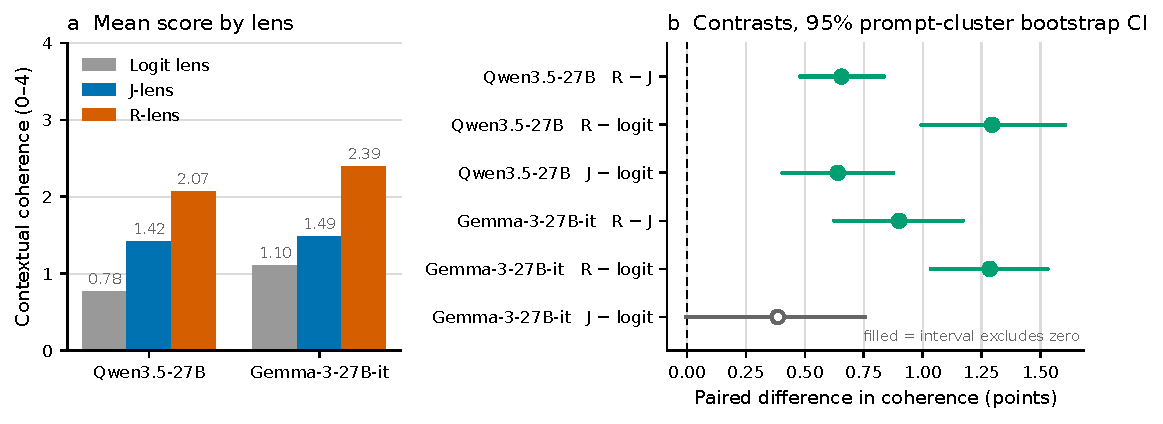
\includegraphics[width=\textwidth]{fig1_primary_result.pdf}
\caption{\textbf{Primary result.} (a) Mean contextual coherence by lens on the
full 0--4 rubric scale. (b) Paired contrasts with 95\% prompt-cluster bootstrap
intervals; a filled marker denotes an interval excluding zero. The axis in (a)
is deliberately not rescaled: the ordering is clear, but every lens sits in the
lower half of the scale.}
\label{fig:primary}
\end{figure}

\subsection{Primary endpoint}

R-Lens is rated more contextually coherent than J-Lens on both models
(Table~\ref{tab:primary}). Both intervals exclude zero in the positive
direction, so the ordering claim replicates on both models.

\begin{table}[h]
\centering
\small
\begin{tabular}{llrrrrrr}
\toprule
Model & Contrast & $\Delta$ & 95\% CI & $p$ & win & tie & loss \\
\midrule
Qwen3.5-27B & R $-$ J        & $0.690$ & \ci{0.515}{0.855} & $<10^{-4}$ & .69 & .20 & .11 \\
Qwen3.5-27B & R $-$ logit    & $0.735$ & \ci{0.475}{0.995} & $<10^{-4}$ & .64 & .12 & .24 \\
Qwen3.5-27B & J $-$ logit    & $0.045$ & \ci{-0.195}{0.275} & $0.771$   & .40 & .19 & .41 \\
\addlinespace
Gemma-3-27B-it & R $-$ J     & $1.010$ & \ci{0.780}{1.240} & $<10^{-4}$ & .76 & .10 & .14 \\
Gemma-3-27B-it & R $-$ logit & $1.440$ & \ci{1.175}{1.680} & $<10^{-4}$ & .80 & .03 & .17 \\
Gemma-3-27B-it & J $-$ logit & $0.430$ & \ci{0.050}{0.795} & $0.115$    & .54 & .06 & .40 \\
\bottomrule
\end{tabular}
\caption{Primary endpoint and the two supporting contrasts, under the
mean-of-two-validated-judges rule. 100 cells and 20 prompts per model. Positive
$\Delta$ favours the first arm.}
\label{tab:primary}
\end{table}

Two features of this table matter as much as the headline.

\textbf{J-Lens is not distinguishable from the logit lens on either model}
($+0.045$, $p = 0.771$ on Qwen; $+0.430$, $p = 0.115$ on Gemma). Under the
primary rule the entire measured advantage over the logit-lens baseline is
carried by the R-Lens variant, not by the Jacobian transport as such. This is a
stronger statement than the adjudicated scoring supports, where the Qwen
J $-$ logit contrast is positive and significant; Section~\ref{sec:judge} shows
the contrast is judge-unstable and should not be quoted as a single number in
either direction.

\textbf{Absolute scores are low.} Mean contextual coherence is 2.07 (Qwen) and
2.39 (Gemma) for R-Lens against 1.42 and 1.49 for J-Lens
(Figure~\ref{fig:primary}a). On this rubric the mid-scale band is
``partially relevant, not a coherent continuation''. R-Lens readouts at
$z \le 0.4$ are better than the alternatives and still not good.

\subsection{Depth}

\begin{figure}[h]
\centering
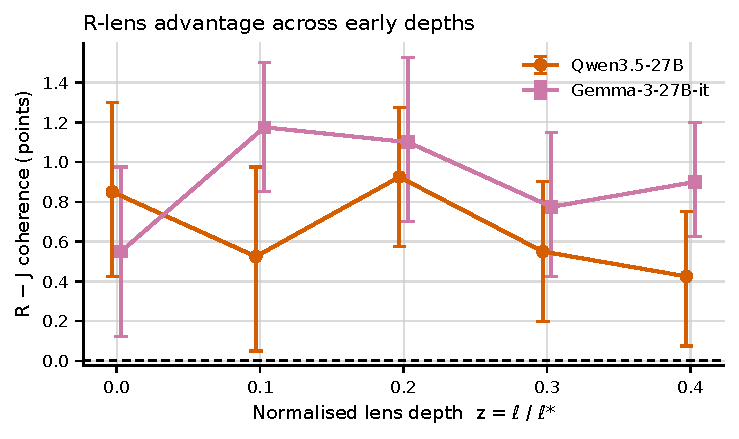
\includegraphics[width=0.62\textwidth]{fig2_depth_profile.pdf}
\caption{\textbf{R $-$ J by normalised depth}, with 95\% intervals. The two
models do not agree on where in depth the advantage is largest.}
\label{fig:depth}
\end{figure}

\flag{The depth profiles disagree between models.} On Qwen the effect is
largest at the embedding layer ($z = 0$, $+0.850$) and decays monotonically to
$+0.425$ by $z = 0.4$. On Gemma the effect at $z = 0$ is the \emph{weakest} of
the five depths ($+0.550$) and the only one that does not survive Holm
correction ($p_{\text{Holm}} = 0.092$); it peaks at $z = 0.1$ ($+1.175$).

A reading on which R-Lens specifically repairs the earliest layers is supported
by Qwen and contradicted by Gemma. What both models support is the weaker
statement that R-Lens is ahead somewhere across $z \le 0.4$.

\subsection{Secondary dimensions}

\begin{table}[h]
\centering
\small
\begin{tabular}{llrr}
\toprule
Model & Dimension (R $-$ J) & $\Delta$ & 95\% CI \\
\midrule
Qwen3.5-27B    & Lexical integrity & $0.125$ & \ci{0.060}{0.190} \\
Qwen3.5-27B    & Prompt echo       & $0.225$ & \ci{0.135}{0.300} \\
Gemma-3-27B-it & Lexical integrity & $0.165$ & \ci{0.035}{0.305} \\
Gemma-3-27B-it & Prompt echo       & $0.305$ & \ci{0.210}{0.395} \\
\bottomrule
\end{tabular}
\caption{Secondary dimensions, both on 0--2 scales.}
\label{tab:secondary}
\end{table}

R-Lens produces more well-formed tokens (lexical integrity) \emph{and} copies
more of the prompt (prompt echo). Both differences exclude zero on both models.
Section~\ref{sec:echo} asks whether the second explains the first.

We do not compare the magnitude of the echo difference to the magnitude of the
coherence difference. They are measured on different scales (0--2 and 0--4) and
such a comparison would be meaningless.

\subsection{By evaluation set}

Per-set differences are all positive on both models and range from $+0.450$
(Qwen, typo) to $+1.900$ (Gemma, poetry). \textbf{No per-set difference
survives Holm correction} ($p_{\text{Holm}} \ge 0.636$ throughout). With four
prompts per set this analysis is descriptive only and is reported for pattern,
not for inference.

\section{Robustness}

\subsection{Integrity audit}

A fail-closed audit re-derived the frozen artifacts from scratch: it recomputed
the panel hash, replayed the per-(cell, rater) arm permutation and compared it
to the key, reconstructed all 400 outgoing judge payloads and scanned them for
lens-identity leakage, and re-parsed every stored judge response.

Twenty conditions were checked. On the first pass nineteen held---including
zero unparseable responses across 526 stored ratings, zero arm-mapping
mismatches, and an exact reproduction of the panel hash
(\texttt{a4984e34\allowbreak{}d835c60e\allowbreak{}cb661552\allowbreak{}ec0a794e}
\dots).

One condition failed, and it was ours. The score-combination rule derived the
combined winner by \emph{voting} on the judges' winners while \emph{averaging}
their scores, which let the two disagree on 18 of 200 cells. The rule was
corrected to derive the winner from the combined scores, and the frozen raw
responses were re-combined without any new API call, so no cell was re-rated and
no rating changed.

\textbf{Re-running the full analysis on the corrected scores changed no reported
number}---all 18 cells were ties under both rules. The audit was then re-run
against the corrected ratings and the analysis those ratings produced, and
\textbf{all twenty conditions pass}, including
\texttt{winner\_matches\_max\_score} across all 200 cells and
\texttt{ratings\_frozen\_before\_analysis}. A defect that changes no number is
still reported here, because whether it changed a number is not something a
reader should have to take on trust.

\subsection{The adjudicator, and why it is not in the primary estimate}
\label{sec:adjudicator}

The original design adjudicated disagreements with a third judge. That judge was
put through the same 78-cell battery as the primaries and cleared eight of nine
gates outright: it never preferred a corrupted arm (0/10), showed no position
bias ($\chi^2 = 0.66$ on 2 df), scored provably-identical arms identically,
returned a tie on 5/5 identity-layer cells, showed full dynamic range on
late-layer controls, and left 0/190 responses unparseable.

It did not clear the order-invariance gate, and---importantly---it did not fail
it either. Rotating the arm order flipped the winner on \textbf{10 of 53
non-tied pairs (18.9\%, 95\% CI \ci{9.4\%}{32.0\%})} against a 15\% ceiling.
An exact binomial test cannot reject 15\% ($p = 0.266$), and the interval is far
too wide to establish that the rate is acceptable. Escalating the battery does
not help: resolving 18.9\% against 15\% at 90\% power needs roughly 810
comparable pairs, a control panel several times the size of the experiment it
exists to validate. For scale, the admitted primary judge GPT-5 scored 1/15
(6.7\%) with an interval of \ci{0.2\%}{32\%}---so this control cannot even
separate the adjudicator from a judge already in use.

\flag{We therefore treated the unresolved gate as a failure and demoted the
adjudicator}, rather than admitting an instrument the battery could not clear or
loosening the threshold to fit it. The primary estimate is the mean of the two
validated judges. The adjudicated estimate is retained below as a sensitivity
analysis, and the adjudicator's ratings are preserved rather than deleted, since
they are evidence about the panel even when not used to score it.

\subsection{Judge dependence}
\label{sec:judge}

\begin{figure}[h]
\centering
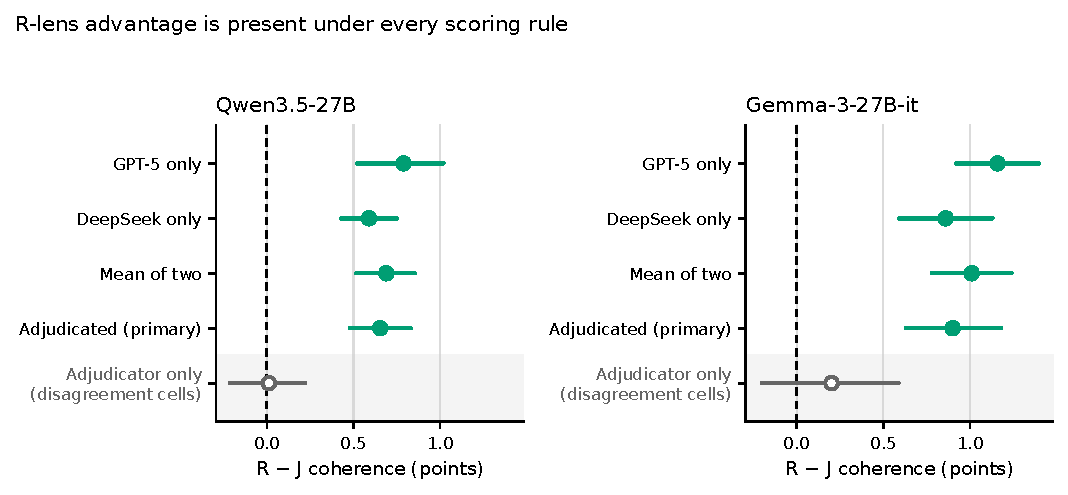
\includegraphics[width=\textwidth]{fig3_judge_sensitivity.pdf}
\caption{\textbf{R $-$ J under four scoring rules.} ``Mean of two'' is the
primary rule; ``Adjudicated'' is the original rule, retained as a sensitivity
analysis after its third judge failed to clear validation. The shaded band is a
diagnostic computed only on cells where the two primary judges disagreed; it is
conditioned on disagreement and is not a fifth estimate of the same quantity.}
\label{fig:judge}
\end{figure}

A two-judge mean is still a scoring rule, and a different rule could give a
different answer. Recomputing under four frozen rules---GPT-5 alone; DeepSeek
alone; the mean of the two (primary); and the original adjudicated rule---gives
a positive R $-$ J on every rule and on both models, with every
individual-judge interval excluding zero. The pooled estimate ranges from
$+0.725$ (DeepSeek alone) to $+0.975$ (GPT-5 alone), with the primary rule at
$+0.850$ and the adjudicated rule at $+0.778$.

The spread across rules (0.25 points pooled) is smaller than the effect itself,
and no rule places the interval anywhere near zero. \textbf{The adjudicated
estimate---the one built on the instrument we demoted---is the smallest of the
four}, so excluding the adjudicator did not manufacture the result; it removed a
conservative influence on it.

\paragraph{The logit-lens contrasts are not stable.}
That verdict is scoped to R $-$ J, and the scoping is load-bearing. Checking
every contrast against the same two single-judge intervals, \flag{five of nine
are not stable across the two primary judges}. On Qwen, GPT-5 rates J-Lens
\emph{significantly worse} than the logit lens ($-0.680$, \ci{-1.06}{-0.33})
while DeepSeek rates it significantly \emph{better} ($+0.770$,
\ci{0.57}{0.97})---same cells, disjoint intervals, opposite signs. Every
unstable contrast involves the logit lens; every R $-$ J contrast is stable.

The natural reading is a floor effect: the judges agree about the relative
ordering of two Jacobian transports and anchor the bottom of a 0--4 scale
differently when asked to score near-noise. Any comparison against the logit
lens in this report should be read with both judges' values in view and must
not be quoted as a single number.

\paragraph{Agreement.} Quadratic-weighted $\kappa = 0.514$ on 600 paired
scores, exact agreement 39.3\%, mean absolute difference 0.91 points. The two
validated judges disagreed on 63\% of cells---the disagreements the third judge
was introduced to settle, and which the primary rule now simply averages over.
\flag{This is moderate agreement at best.} With validated judges it is evidence
about the material rather than the instrument---the readouts being rated are
genuinely ambiguous, which is what one expects of early-layer readouts---but a
$\kappa$ of 0.51 is not a precise instrument, and every interval in this
document inherits that noise.

\subsection{Prompt echo}
\label{sec:echo}

\begin{figure}[h]
\centering
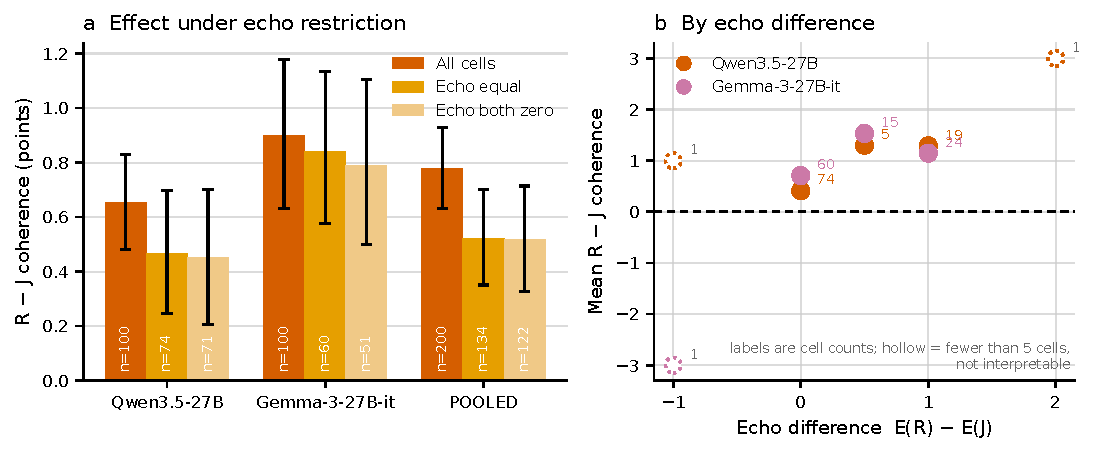
\includegraphics[width=\textwidth]{fig4_echo_sensitivity.pdf}
\caption{\textbf{Echo sensitivity.} (a) R $-$ J restricted by echo agreement,
retained cell counts printed inside each bar. (b) Mean R $-$ J by echo
difference; labels are cell counts and hollow markers mark strata too small to
interpret.}
\label{fig:echo}
\end{figure}

R-Lens copies more of the prompt than J-Lens, and a rater who rewards
prompt-shaped text would score it higher for that reason alone. Restricting to
cells where both lenses received the \emph{same} echo score:

\begin{table}[h]
\centering
\small
\setlength{\tabcolsep}{4pt}
\begin{tabular}{lrrrrr}
\toprule
Model & All cells & Echo equal & retained & Echo both zero & retained \\
\midrule
Qwen3.5-27B    & $0.690$ & $0.509$ \ci{0.30}{0.72} ($n{=}68$) & 74\% & $0.526$ \ci{0.29}{0.76} ($n{=}62$) & 76\% \\
Gemma-3-27B-it & $1.010$ & $1.031$ \ci{0.70}{1.40} ($n{=}53$) & 102\% & $1.083$ \ci{0.75}{1.46} ($n{=}36$) & 107\% \\
Pooled         & $0.850$ & $0.577$ \ci{0.45}{0.70} ($n{=}121$) & 68\% & $0.686$ \ci{0.49}{0.90} ($n{=}98$) & 81\% \\
\bottomrule
\end{tabular}
\caption{R $-$ J contextual coherence under echo restriction, frozen
mean-of-two scoring. ``Retained'' is the restricted estimate as a percentage
of the all-cells estimate; it can exceed 100\%, as it does on Gemma, where
matching on echo does not shrink the effect at all.}
\label{tab:echo}
\end{table}

The effect survives in all 24 subset estimates---every scoring variant, both
models, both restriction rules---with intervals excluding zero throughout.
\flag{But roughly a third of the pooled gap coincides with an echo difference}
under the equal-echo restriction, and the pattern is not uniform: on Qwen the
estimate falls by about a quarter, while on Gemma it does not fall at all.
The Gemma both-zero cell retains only 36 cells from 17 prompts and its interval
is correspondingly wide; it should not be read as evidence that echo is
irrelevant there.

\paragraph{This is not a causal adjustment.} Echo is measured from the same
readouts as coherence, so restricting on it conditions on a post-treatment
variable. The regression of the coherence difference on the echo difference is
descriptive; its intercept is the fitted difference at equal echo, not an
echo-adjusted effect. \flag{The two judges also disagree about the mechanism}:
GPT-5's slope is $\approx 1.0$--$1.1$ with intervals excluding zero on both
models, while DeepSeek's is $0.29$ \ci{-0.16}{0.80} and $0.35$
\ci{-0.03}{0.63}, both covering zero. GPT-5 sees echo and coherence tightly
coupled; DeepSeek sees almost no coupling. Both still rate R above J.

\paragraph{What would settle it.} A rubric that scores coherence
\emph{excluding} copied spans, validated against controls in which a pure
prompt-copy arm must not win, would test this directly rather than by
restriction. That instrument is specified but not yet run.

\subsection{Judge behaviour}

\begin{figure}[h]
\centering
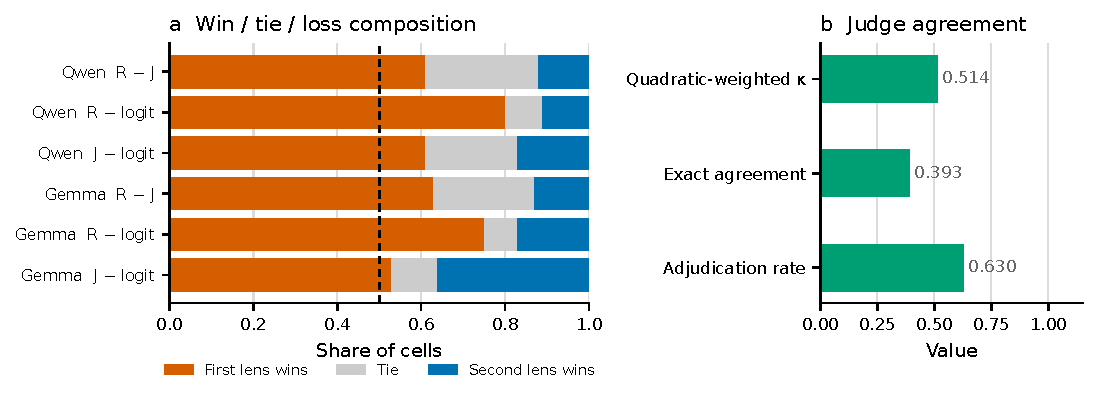
\includegraphics[width=\textwidth]{fig5_judge_agreement.pdf}
\caption{\textbf{What the judges did.} (a) Win/tie/loss composition per
contrast. (b) Agreement statistics. A mean difference of 0.78 points is
compatible with very different underlying distributions; the composition shows
which.}
\label{fig:agreement}
\end{figure}

R-Lens wins 61--63\% of R $-$ J cells and loses 12--13\%, with the remaining
quarter tied. The effect is a broad shift, not a handful of extreme cells.

\section{The earlier no-prompt panel}

An earlier 50-cell panel on Qwen returned a null for R $-$ J ($+0.080$, 95\% CI
\ci{-0.16}{0.34}, $p = 0.596$). It is reported here for completeness and is
\textbf{not comparable} to the present result. The two panels differ
simultaneously in prompt visibility (that panel did not show raters the prompt),
size (50 vs 200 cells), rubric scale, judge count, sampling rule and
adjudication, and one of its raters was contaminated. No single one of those
differences can be identified as the reason the results differ, and we do not
claim to know which mattered. It is a preliminary attempt that was superseded,
not a contradicting measurement.

That panel did produce one durable negative result, obtained against 150 human
judgements: of three cheap token-form proxies for coherence, only the
``trash-rate'' proxy correlated in the expected direction ($\rho = -0.640$).
Zero-corpus-frequency rate ($\rho = +0.330$) and in-prompt rate
($\rho = -0.245$) were both \emph{inverted}, retracting two earlier readings of
ours. Token-form statistics are not a substitute for rating the readouts.

\section{Limitations}

\begin{enumerate}[leftmargin=*]
\item \textbf{One judge was demoted, not merely unused.} The adjudicator
      cleared 8 of 9 validation gates but its order-invariance rate
      (18.9\%, \ci{9.4\%}{32.0\%}) could neither be admitted nor rejected by a
      feasible battery. We excluded it. A reader who would have admitted it
      should read the adjudicated row of Figure~\ref{fig:judge} as the headline
      instead; it is smaller ($+0.778$ pooled) and still excludes zero.
\item \textbf{Order invariance is weakly controlled for every judge.} The same
      battery gives GPT-5 an interval of \ci{0.2\%}{32\%}. The control is too
      blunt at this size to certify any of the three judges tightly, and a
      larger one was judged not worth its cost.
\item \textbf{Released lenses use the 25-prompt light recipe}, not the
      1000-prompt recipe of the source post. Effect sizes are not comparable to
      the authors'.
\item \textbf{Twenty prompts per model.} Adequate for the pooled estimand,
      which is why intervals are prompt-clustered; not adequate for the
      per-set breakdown, which is descriptive only.
\item \textbf{Autoraters, not humans.} No human panel was run. Judges were
      validated against controls, but LLM raters may share biases with each
      other and with the models being read.
\item \textbf{Echo is not causally controlled}, only restricted on.
\item \textbf{Logit-lens comparisons are judge-dependent} and should not be
      quoted as single numbers.
\item \textbf{Depth-localisation does not replicate across models.}
\item \textbf{Ordering, not quality.} Nothing here shows early-layer R-Lens
      readouts are coherent in absolute terms; they average roughly 2 of 4.
\end{enumerate}

\section{What would change the conclusion}

\begin{itemize}[leftmargin=*]
\item The adjudicator failing its validation battery would not overturn the
      direction, but would demote the adjudicated estimate and promote the
      mean-of-two.
\item A non-echo rubric---coherence scored excluding copied spans---returning a
      null would move the reading from ``R-Lens reads out more coherently'' to
      ``R-Lens copies the prompt more, and raters reward that''.
\item A human panel disagreeing with the autoraters at scale would invalidate
      the instrument, not merely widen the intervals.
\item Refitting both lenses at $n = 1000$ and finding the gap disappears would
      indicate the effect is a property of the light recipe.
\end{itemize}

\section{Reproducibility}

Every number in this document is produced by a command in the repository
operating on frozen artifacts; none is transcribed by hand into a plotting
script or a table. The figures are drawn by \texttt{rlens figures} directly from
the analysis outputs, and skip themselves by name if an input is missing rather
than falling back to defaults.

\begin{center}
\small
\begin{tabular}{ll}
\toprule
Stage & Command \\
\midrule
Preflight (fail-closed)      & \texttt{rlens preflight} \\
Prompt selection             & \texttt{rlens eligibility} \\
Panel freeze                 & \texttt{rlens freeze-panel}, \texttt{rlens panel-v2} \\
Judge validation             & \texttt{rlens judge-validate} \\
Rating                       & \texttt{rlens autorate} \\
Primary analysis             & \texttt{rlens analyse-v2} \\
Integrity audit              & \texttt{rlens audit-v2} \\
Judge and echo sensitivity   & \texttt{rlens robustness} \\
Figures                      & \texttt{rlens figures} \\
\bottomrule
\end{tabular}
\end{center}

\begin{sloppypar}
\noindent
Artifact hashes, the protocol salt, seeds and the audit verdicts are recorded in
\texttt{final\_reproducibility\_\allowbreak manifest.json}. The unblinding key is
deliberately absent from the repository and from this document's source tree.
\end{sloppypar}

\end{document}
